\chapter{Data and Methodology}
\label{chap:data_methodology}

\section{The ICIJ Offshore Leaks Database as "proxy" (EU, 2017 paper): Structure, Content, Strengths, Limitations (Nodes, Relationships, Leaks included, \texttt{sourceID}, \texttt{valid\_until}, incompleteness).} % Used \texttt for code-like terms
\label{sec:3_1}
\begin{itemize}[leftmargin=*]
    \item Numerical estimates will surely be biased, but the qualitiative nature of intereactions less so
\end{itemize}

\section{External Data Sources: Country-Level Indicators (WJP RoL, TI CPI, Regime Type, GDP, etc.), Jurisdiction-Level Data (FSI, Regulatory status).}
\label{sec:3_2}
Lafitte 2024: Legal innovatoins

Laffitte, S. (2024). The Historical Tax Havens Database (HTHD).

World Justice Project (WJP) Rule of Law Index.

VDEM Regime Type Data.
Coppedge, Michael, John Gerring, Carl Henrik Knutsen, Staffan I. Lindberg, Jan Teorell, David Altman, Fabio Angiolillo, Michael Bernhard, Agnes Cornell, M. Steven Fish, Linnea Fox, Lisa Gastaldi, Haakon Gjerløw, Adam Glynn, Ana Good God, Sandra Grahn, Allen Hicken, Katrin Kinzelbach, Joshua Krusell, Kyle L. Marquardt, Kelly McMann, Valeriya Mechkova, Juraj Medzihorsky, Natalia Natsika, Anja Neundorf, Pamela Paxton, Daniel Pemstein, Johannes von Römer, Brigitte Seim, Rachel Sigman, Svend-Erik Skaaning, Jeffrey Staton, Aksel Sundström, Marcus Tannenberg, Eitan Tzelgov, Yi-ting Wang, Felix Wiebrecht, Tore Wig, Steven Wilson and Daniel Ziblatt. 2025. "V-Dem [Country-Year/Country-Date] Dataset v15" Varieties of Democracy (V-Dem) Project. \url{https://doi.org/10.23696/vdemds25} % Added \url

\begin{itemize}[leftmargin=*]
    \item World Inequality Database with data on wealth inequality.
\end{itemize}

\section{Using Agentic AI to Scrape data on intermediaries.}
\label{sec:3_3}
Using an AI-loop to classify the type of intermediary.
ICIJ data just classifies them generically. For our purposes, it is useful to get more information on them, and put them into the typology from the EU (2017) paper.

% Placeholder for figure: Make sure you have 'agent_loop_diagram.png' in your 'images' folder
\begin{figure}[htbp]
    \centering
    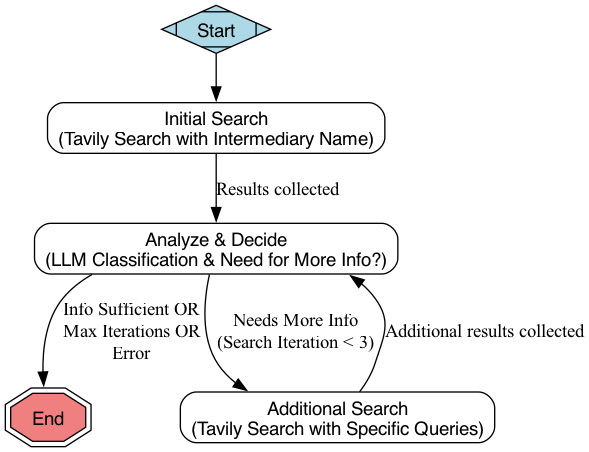
\includegraphics[width=0.8\textwidth]{agent_graph.png}
    \caption{Basic Agent Loop for Intermediary Classification}
    \label{fig:agent_loop_placeholder}
\end{figure}

In brief, an AI-agent orchestrates searches for these people, online first gneerically reading the results, then coming up with more specific ones based on the information it discovers or lacks, searching up to 3 queries, and scouring 15 most relevant results based on query-result embedding similiarity (Tavily). Effectively, replaces the need for individually searching for each person

For each, it then classifies it accordingly with a few additional fields as well as listing the confidecne of its judgement.

There are a few obvious issues with such a proposal, that I wish to assuage

\textbf{Temporally misaligned}
All of the seraches necessarily today, and on the information found htere.
\begin{enumerate}[label=\arabic*.]
    \item This immediately biases it otwrads those intermeidaries that are more current, and
    \item retrospectively assumes that the role they played then is equivalent to what one gets when one scours them today.
\end{enumerate}
This issues aren't too big however. To the first point, there isn't an obvious reason why this should be a problem beyond limiting power. If we can only identify 50\% of them, so be it. This only becomes problematic if there should be a systematic bias in the way it's used. E.g. it's easier to identify tax experts compared to legal experts, one may ofr exampel have a reason to stay more covert. This is when it becomes a very real threat to any potnetial infernece.

To the second, this shuoldn't be too bad a problem either. Most firms/individuals woudl likely not switch between these roles, considering the highly specialised nature of each of the functios and the considerable barriers to entry to each.

\textbf{General trouble with using LLMs}
Certainly there is also issue with using large-language models as a substitute for human annotation and research. This is experimental, but similar processes have been used to great effect in e.g. (INSERT SOME CITATION HERE).

If there is a systematic direction of bias, I cannot think of it.
